% $Header$

\documentclass[t,14pt,mathserif]{beamer}

% This file is a solution template for:

% - Talk at a conference/colloquium.
% - Talk length is about 20min.
% - Style is ornate.



% Copyright 2004 by Till Tantau <tantau@users.sourceforge.net>.
%
% In principle, this file can be redistributed and/or modified under
% the terms of the GNU Public License, version 2.
%
% However, this file is supposed to be a template to be modified
% for your own needs. For this reason, if you use this file as a
% template and not specifically distribute it as part of a another
% package/program, I grant the extra permission to freely copy and
% modify this file as you see fit and even to delete this copyright
% notice.


% Copyright 2012 by Aécio S. R. Santos <aecio.solando@gmail.com>.
%
% In principle, this file can be redistributed and/or modified under
% the terms of the GNU Public License, version 2.
%
% However, this file is supposed to be a template to be modified
% for your own needs. For this reason, if you use this file as a
% template and not specifically distribute it as part of a another
% package/program, I grant the extra permission to freely copy and
% modify this file as you see fit and even to delete this copyright
% notice. 

% Redefins a fonte
\usepackage{helvet}

% Define some colors...
\definecolor{titlecolor}{rgb}{0, 0.37, 0.59}
\definecolor{lightblue}{rgb}{.0, .68, .84}
\definecolor{black}{rgb}{0, 0, 0}
\definecolor{gray}{rgb}{0.3, 0.3, 0.3}

% Remove these comments for green color scheme
%\definecolor{titlecolor}{rgb}{0, 0.5, 0.48}
%\definecolor{lightblue}{rgb}{0.2,0.2,0.7}

% Define color of alert text
\setbeamercolor{alerted text}{fg=lightblue}

% Define tamanho das fontes
\setbeamerfont{frametitle}{parent=structure,size=\Large}
\setbeamerfont{framesubtitle}{parent=frametitle,size=\footnotesize}
\setbeamerfont{itemize/enumerate body}{size=\fontsize{16pt}{17.6pt}}
\setbeamerfont{itemize/enumerate subbody}{size=\fontsize{14pt}{15,4pt}}
\setbeamerfont{itemize/enumerate subsubbody}{size=\footnotesize}

% Redefine a fonte do titulo da capa como negrito
%\setbeamerfont{title}{size=\Large, series=\bfseries}

% Redefine cover title color
\setbeamercolor{title}{fg=titlecolor}

% Redefine title color
\setbeamercolor{frametitle}{fg=titlecolor,size=20pt}

% Uncomment to redefine bullets with round format
%\useinnertheme[shadow]{rounded}
%\setbeamertemplate{blocks}[rounded][shadow=\beamer@themerounded@shadow]
%\setbeamertemplate{items}[ball]

% Redefine bullets color
\setbeamercolor*{item}{fg=lightblue}

% Redefine spacing of left margin of bullets
\setlength{\leftmargini}{1.3em}
\setlength{\leftmarginii}{1em}
\setlength{\leftmarginiii}{1em}

% Redefine space between of items in 'itemize' enviroment
\newlength{\wideitemsep}
\setlength{\wideitemsep}{\itemsep}
\addtolength{\wideitemsep}{0.25pt}
\let\olditem\item
\renewcommand{\item}{\setlength{\itemsep}{\wideitemsep}\olditem}

% Redefine space before a nested itemize
\makeatletter
\def\@listii{\leftmargin\leftmarginii
              \topsep    0.9ex
              \parsep    0\p@   \@plus\p@
              \itemsep   \parsep}
\makeatother


% Redefine width of text area margins
\setbeamersize{text margin left=1em,text margin right=1em}

% Define summary items depth
\setcounter{tocdepth}{2}

% Redefine styles of frames' title
\setbeamertemplate{frametitle} {
  \vspace{0.2cm}
  \ifbeamercolorempty[bg]{frametitle}{}{\nointerlineskip}%
  \begin{beamercolorbox}[]{frametitle}
    \ifbeamercolorempty[bg]{frametitle}{}{\nointerlineskip}%
    \usebeamerfont{frametitle}{%
      \strut\insertframetitle\strut\par%
    }
    {%
      \ifx\insertframesubtitle\@empty%
      \else
  \usebeamerfont{framesubtitle}\usebeamercolor[fg]{framesubtitle}\insertframesubtitle\strut\par
      \fi
      \vspace{-.9cm}%
      {
  \textcolor{gray} {\rule[5pt]{\linewidth}{.5pt}\vspace{-8pt}}
      }
    }%  
    \vskip-0.5ex%
    \if@tempswa\else\vskip-.9cm\fi
  \end{beamercolorbox}%
  \vspace{0.2cm}
}

% Removes navigation bar
\beamertemplatenavigationsymbolsempty 

% Redefine footline to show only slide number
\setbeamertemplate{footline}{
  \begin{beamercolorbox}[wd=1\paperwidth,ht=2.25ex,dp=1ex,right]{date in head/foot}%
    %\hfill
    \insertframenumber{}                             % Only current slide number
    %\insertframenumber{} / \inserttotalframenumber  % Current slide number and total of slides
    \hspace{2ex} 
  \end{beamercolorbox}
}

\usepackage[brazil]{babel}
%\usepackage[english]{babel}

\usepackage{graphicx}   %Package para figuras
% or whatever

\usepackage[utf8]{inputenc}
% or whatever

\usepackage{times}
\usepackage[T1]{fontenc}
\usepackage{tabularx}
\usepackage{multirow}
\usepackage{adjustbox}
\usepackage{array}
%\usepackage[cmex10]{amsmath}
% Or whatever. Note that the encoding and the font should match. If T1
% does not look nice, try deleting the line with the fontenc.

\newcommand{\semitransp}[2][35]{\color{fg!#1}#2}

\title[] % (optional, use only with long paper titles)
{Ferramentas para Business Report \\
com Suporte à Linguagem XBRL - \\
Revisão Sistemática da Literatura}

\subtitle
{Vagner Clementino}

%\author[] % (optional, use only with lots of authors)
%{Vagner Clementino~\inst{1}} %\and S.~Another\inst{2}}
% - Give the names in the same order as the appear in the paper.
% - Use the \inst{?} command only if the authors have different
%   affiliation.

\institute[] % (optional, but mostly needed)
{
%  \inst{1}%
  Departamento de Ciência da Computação\\
  Universidade Federal de Minas Gerais (UFMG)\\
  Empirical Software Engineering - 2015\\
  %\and
  %\inst{2}%
  %Department of Theoretical Philosophy\\
  %University of Elsewhere
  }
% - Use the \inst command only if there are several affiliations.
% - Keep it simple, no one is interested in your street address.

\date[2015/12/16] %o(optional, should be abbreviation of conference name)
%{Software Quality and Measurement 2015-1 \\Prof. Eduardo Figueiredo}
% - Either use conference name or its abbreviation.
% - Not really informative to the audience, more for people (including
%   yourself) who are reading the slides online

\subject{Software Engineer}
% This is only inserted into the PDF information catalog. Can be left
% out.



% If you have a file called "university-logo-filename.xxx", where xxx
% is a graphic format that can be processed by latex or pdflatex,
% resp., then you can add a logo as follows:

% \pgfdeclareimage[height=0.5cm]{university-logo}{university-logo-filename}
% \logo{\pgfuseimage{university-logo}}



% Delete this, if you do not want the table of contents to pop up at
% the beginning of each subsection:
\AtBeginSubsection[]
{
  \begin{frame}<beamer>{Outline}[allowframebreaks]
    \tableofcontents[currentsection,currentsubsection]
  \end{frame}
}


% If you wish to uncover everything in a step-wise fashion, uncomment
% the following command:

%\beamerdefaultoverlayspecification{<+->}

\expandafter\def\expandafter\insertshorttitle\expandafter{%
  \insertshorttitle\hfill%
  \insertframenumber\,/\,\inserttotalframenumber}

\setbeamertemplate{caption}[numbered]
\setbeamertemplate{bibliography item}{\insertbiblabel}
\begin{document}

\begin{frame}
  \titlepage
\end{frame}

\begin{frame}{Outline}
  \tableofcontents
  % You might wish to add the option [pausesections]
\end{frame}


% Structuring a talk is a difficult task and the following structure
% may not be suitable. Here are some rules that apply for this
% solution:

% - Exactly two or three sections (other than the summary).
% - At *most* three subsections per section.
% - Talk about 30s to 2min per frame. So there should be between about
%   15 and 30 frames, all told.

% - A conference audience is likely to know very little of what you
%   are going to talk about. So *simplify*!
% - In a 20min talk, getting the main ideas across is hard
%   enough. Leave out details, even if it means being less precise than
%   you think necessary.
% - If you omit details that are vital to the proof/implementation,
%   just say so once. Everybody will be happy with that.
\section{Introdução}
\begin{frame}{Introdução}
    \begin{itemize}
      \item Organizações estão se tornando cada vez mais transparentes com
        relação às suas operações
      \item Informações são disponibilizadas aos stakeholders através de
        Relatórios de Negócio (Business Report)

    \end{itemize}
\end{frame}

\begin{frame}{Introdução}
    \begin{itemize}
      \item No Brasil, o processo de transparência dos entes públicos ainda têm
        o que melhorar
       \item Escala Brasil Transparente\footnote{Disponível em \url{http://www.cgu.gov.br/assuntos/transparencia-publica/escala-brasil-transparente}}
    \end{itemize}

\begin{figure}[htb]
\centering
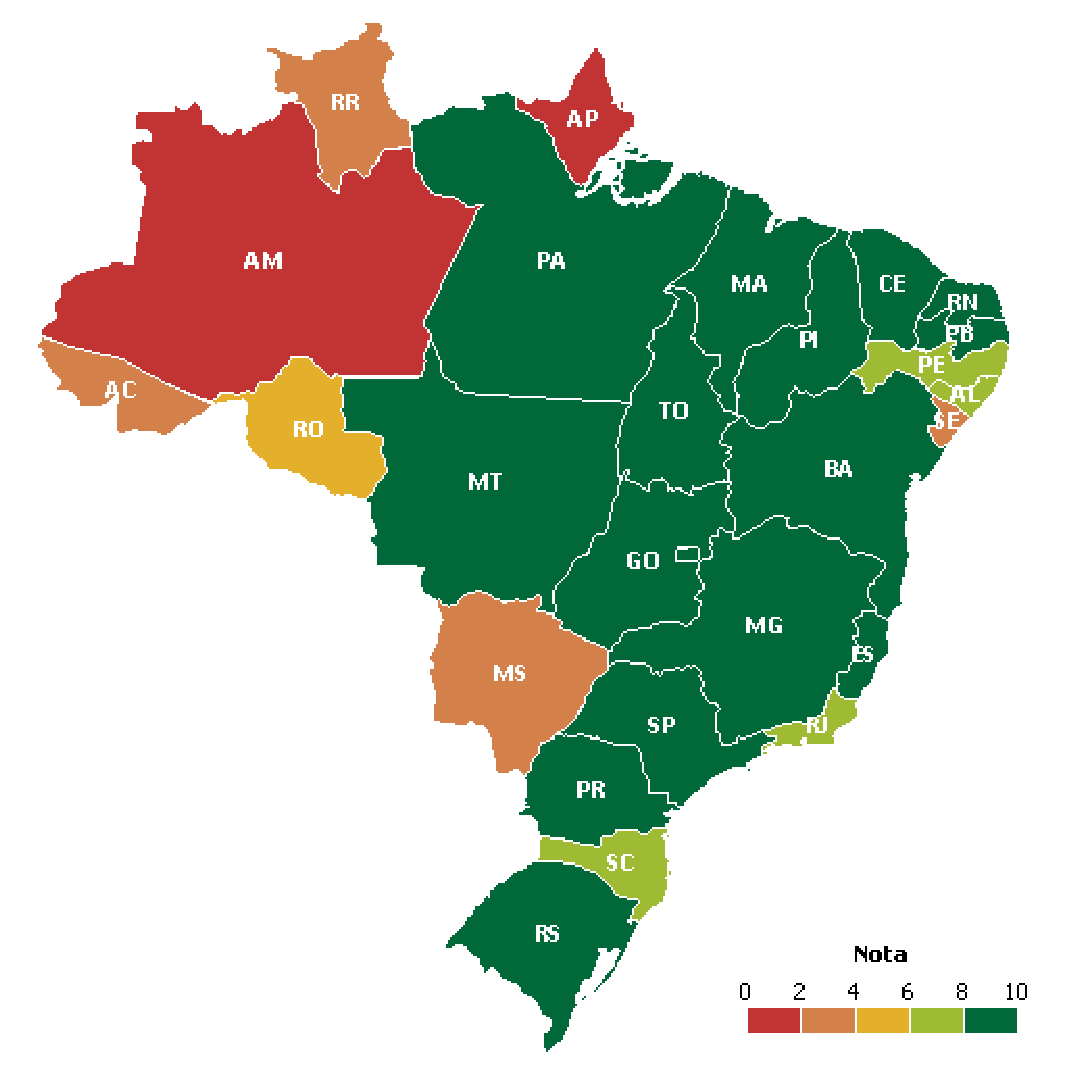
\includegraphics[width=.357\textwidth]{../img/ebt.eps}
\end{figure}
\end{frame}

\section{Background}
\begin{frame}{eXtensible Business Report Language - XBRL}

    \begin{itemize}
      \item \alert{XBRL} é uma linguagem para divulgação e intercâmbio de
        informações financeiras baseada em XML, conforme Silva et. al.\cite{xbrl_conceitos_aplicacoes}.
      \item Baseada nos conceitos de \alert{Taxonomia} e \alert{Documentos de Instância}
    \end{itemize}
\end{frame}
%%%%%%%%%%%%%%%%%%%%%%%%%%%%%%%%%%%%%%%
\begin{frame}{Taxonomia em XBRL}
    \begin{figure}[htb]
\centering
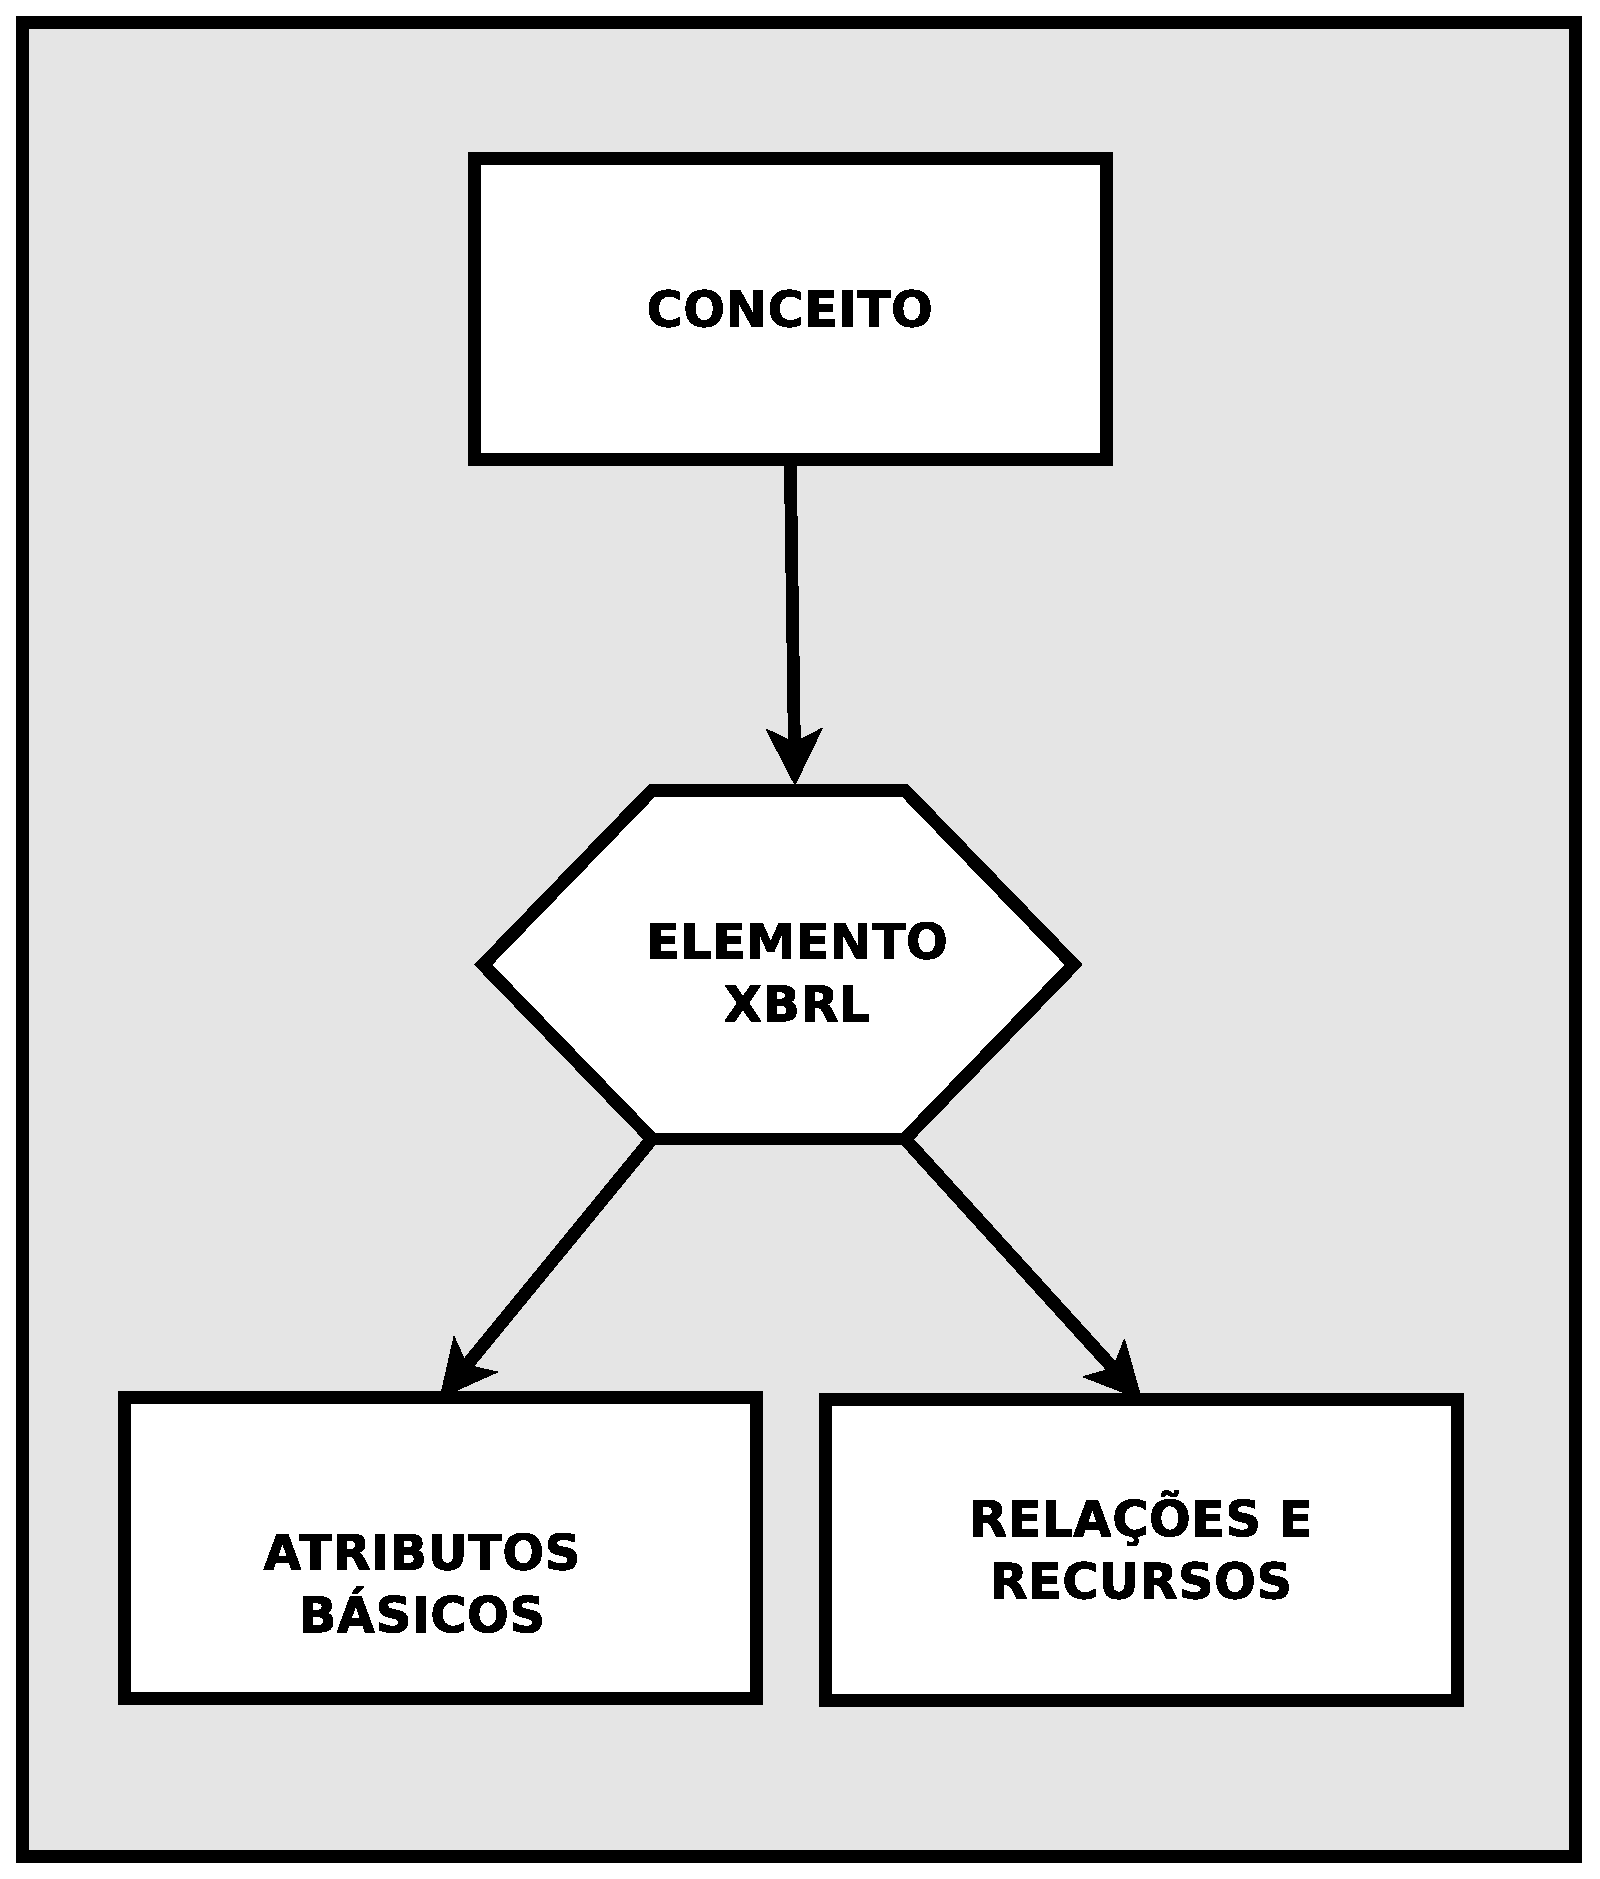
\includegraphics[width=.357\textwidth]{../img/taxonomia.eps}
\end{figure}
\end{frame}
%%%%%%%%%%%%%%%%%%%%%%%%%%%%%%%%%%%%%

\begin{frame}{Exemplo de Documento XBRL}
\begin{figure}[htb]
\centering
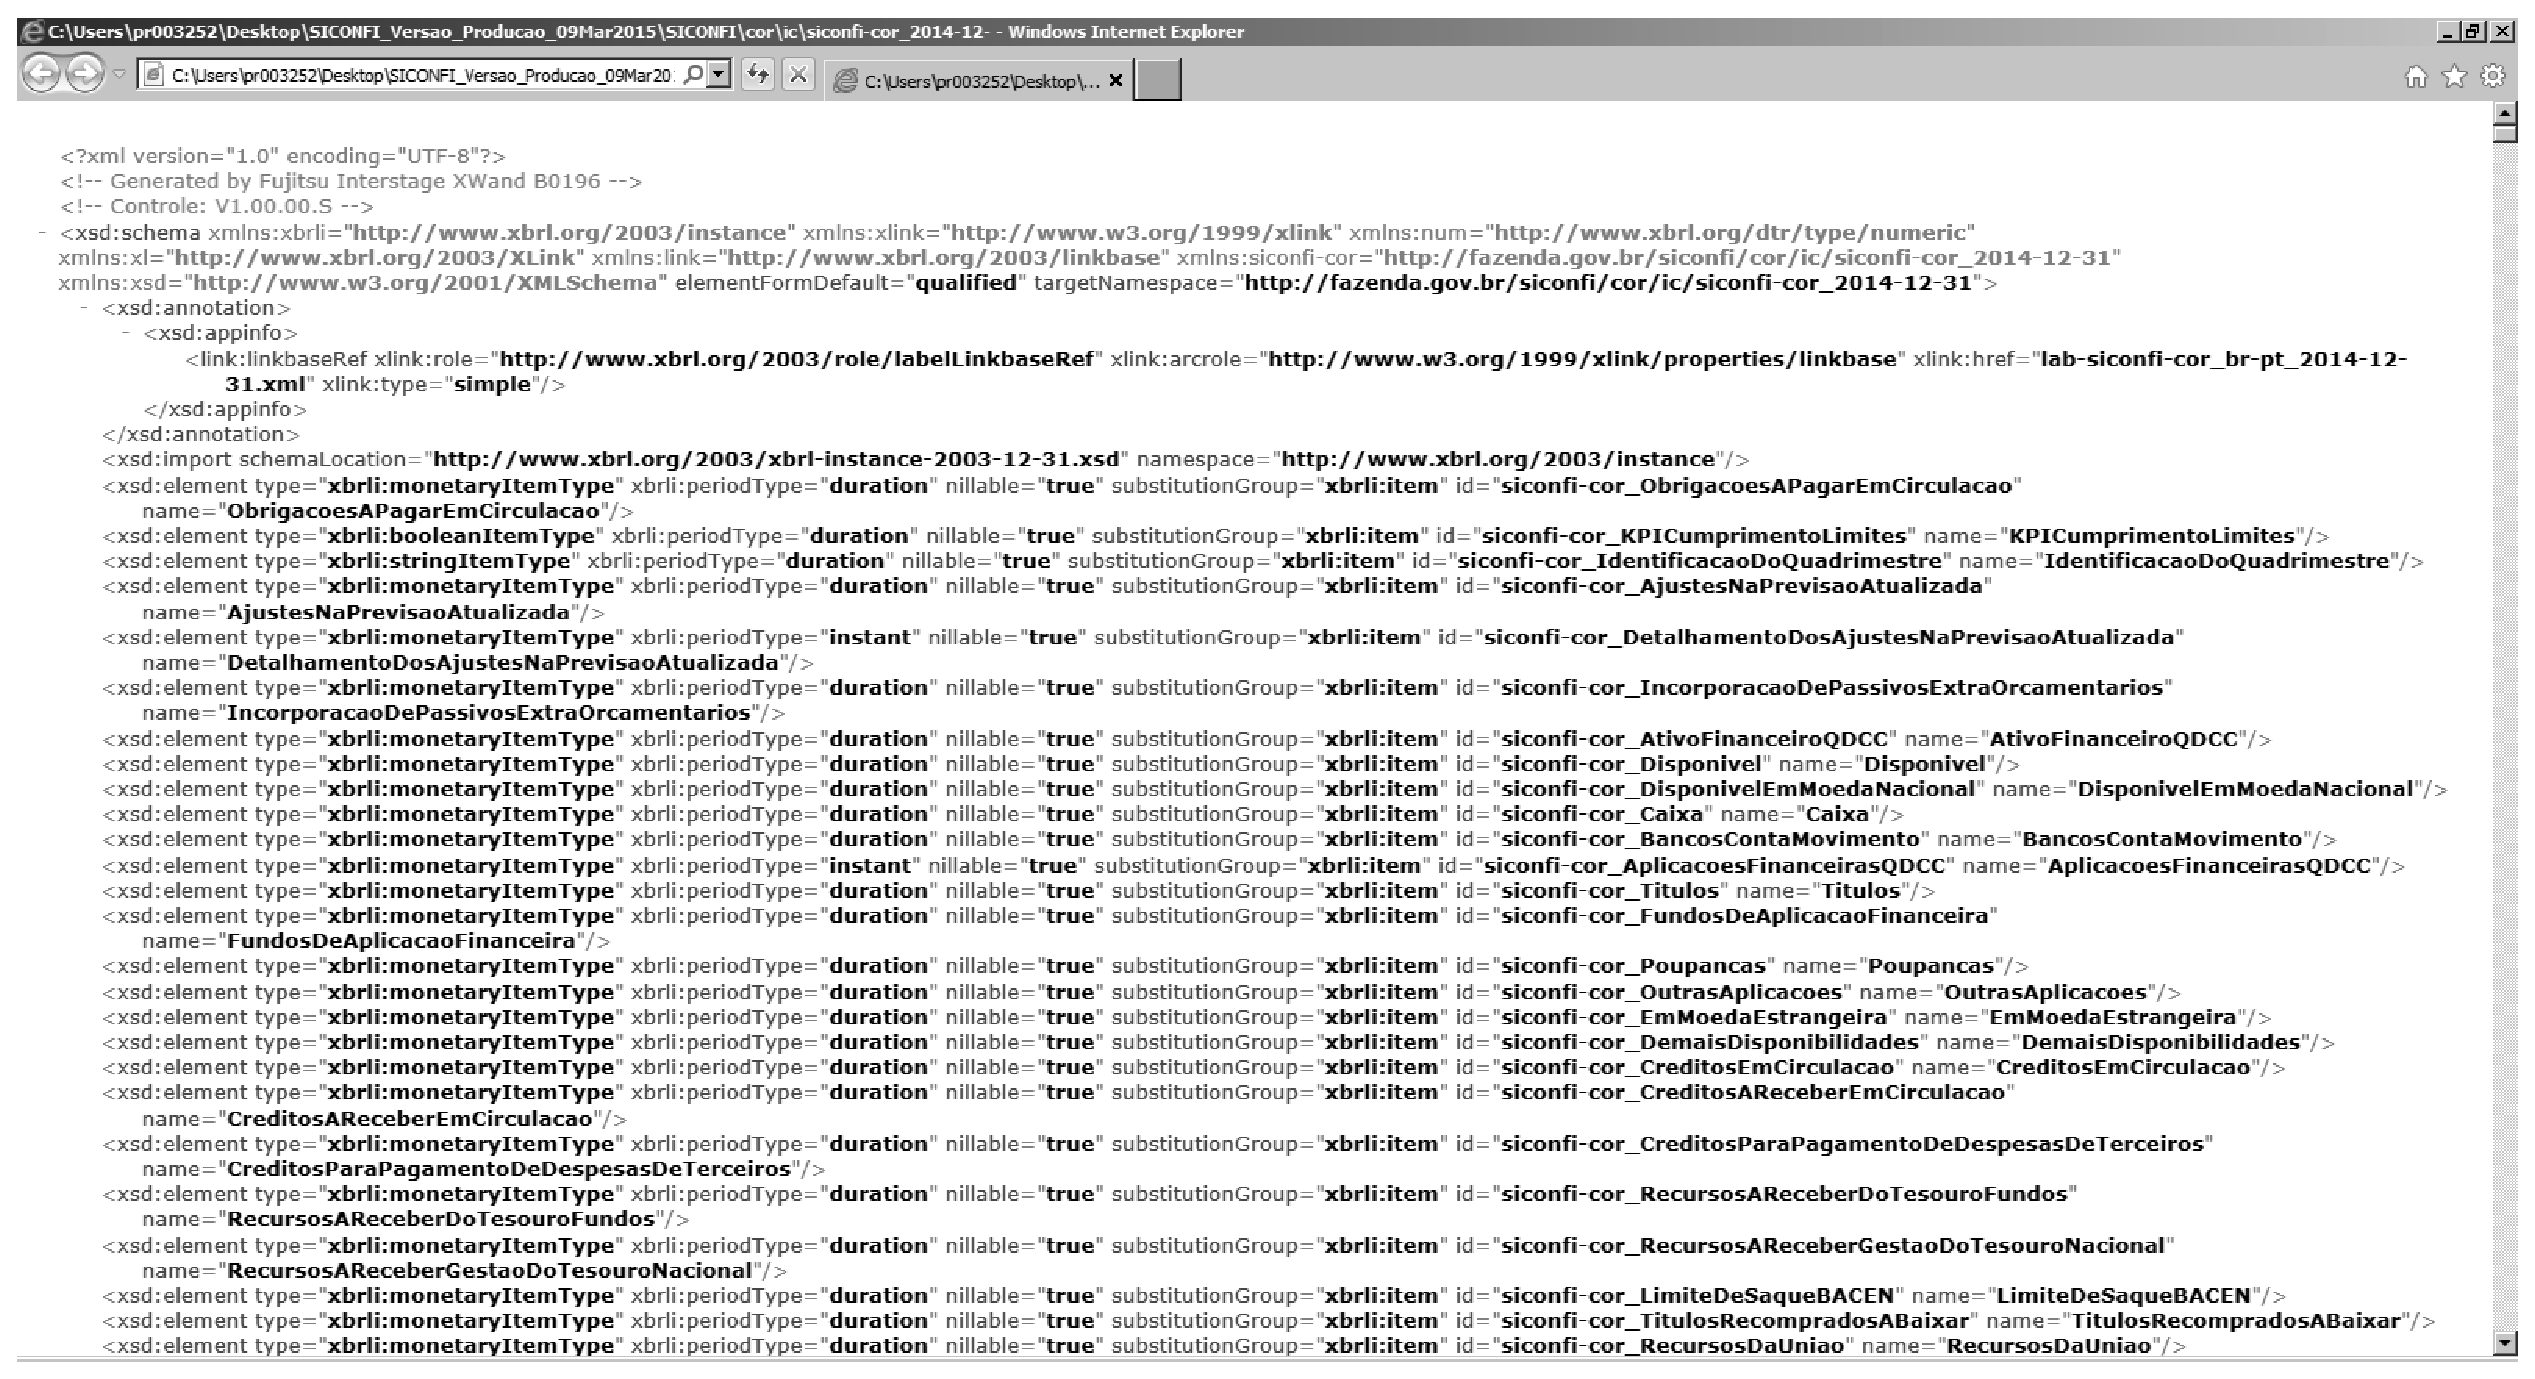
\includegraphics[width=\textwidth]{../img/arquivo_xsd.eps}
\end{figure}
\end{frame}
%%%%%%%%%%%%%%%%%%%%%%%%%%%%%%%%%%%%%
\begin{frame}{Relatórios  de Negócio (Business Report)}
    \begin{itemize}
      \item Segundo Lymer et al.\cite{lymer1999business} é o produto final da divulgação
        pública de dados operacionais e financeiros de uma organização
      \item Prestação regular de informações para os gestores para tomada de decisão.
      \item Exemplos
      \begin{itemize}
           \item Capital Requirements Directives (CRD)
           \item Matriz de Saldos Contábeis
           \item Gastos com pessoal do governo federal
      \end{itemize}

    \end{itemize}
\end{frame}

\section{Justificativa}
\begin{frame}{Justificativa}
    \begin{itemize}
      \item Secretaria do Tesouro Nacional definiu o XBRL como padrão para o
        envio de relatórios de prestação de contas.
      \item Demanda por parte das organizações de referências de qualidade
        sobre o assunto de \textit{XBRL}.
      \item \textit{Subsidiar a tomada de decisão} sobre a aquisição ou
        desenvolvimento de ferramentas de suporte à XBRL.
  \end{itemize}
\end{frame}

\section{Objetivo}
\begin{frame}{Objetivo do Trabalho}
    \begin{itemize}
      \item Revisar a bibliografia de Engenharia de Software a fim de descobrir
        ferramentas para Relatórios de Negócio com suporte à XBRL, suas
        funcionalidades e área de atuação.
  \end{itemize}
\end{frame}

\section{Metodologia}
%%%%%%%%%%%%%%%%%%%%%%%%%%%%%%%%%%%%%%%%%%%%%%%%%%%%%%%%
\begin{frame}{Protocolo da Revisão}
    \begin{itemize}
      \item Definição de um Protocolo com diretrizes para SLR, conforme
        Kitchenham et. al. \cite{kitchenham2009systematic}
      \item Foram propostas Questões de Pesquisa a serem respondidas pela SLR
  \end{itemize}
\end{frame}
%%%%%%%%%%%%%%%%%%%%%%%%%%%%%%%%%%%%%%%%%%%%%%%%%%%%%%%%%
%%%%%%%%%%%%%%%%%%%%%%%%%%%%%%%%%%%%%%%%%%%%%%%%%%%%%%%%
\begin{frame}{Questões de Pesquisa}
    \begin{itemize}
     \item \textbf{$Q1$}: Quais são as ferramentas para Relatórios de Negócio que
    suportam a XBRL?
  \item \textbf{$Q2$}: Quais são as funcionalidades comuns as ferramentas
    que possibilitem a comparação entre elas?
    \end{itemize}
\end{frame}
%%%%%%%%%%%%%%%%%%%%%%%%%%%%%%%%%%%%%%%%%%%%%%%%%%%%%%%%%
%%%%%%%%%%%%%%%%%%%%%%%%%%%%%%%%%%%%%%%%%%%%%%%%%%%%%%%%
\begin{frame}{Questões de Pesquisa}
    \begin{itemize}
        \item \textbf{$Q3$}: Existem casos reais de utilização da ferramenta
    (Estudos de Casos, Whitepapers e etc)?
      \item \textbf{$Q4$}: Qual setor da economia (governos, medicina, setor financeiro) a ferramenta possui histórico de utilização?
    \end{itemize}
\end{frame}
%%%%%%%%%%%%%%%%%%%%%%%%%%%%%%%%%%%%%%%%%%%%%%%%%%%%%%%%%
%%%%%%%%%%%%%%%%%%%%%%%%%%%%%%%%%%%%%%%%%%%%%%%%%%%%%%%%
\begin{frame}{Critérios de Inclusão e Exclusão}
    \begin{itemize}
      \item Critérios de \textit{inclusão}
              \begin{itemize}

                   \item Publicado a partir de 2008.
                   \item Estar escrito em língua inglesa.
                   \item Artigos de Conferência, journals e Whitepapers
                   \item Dissertações ou Teses apenas se a ferramenta proposta tenha sido
  implementada e testada.
              \end{itemize}
    \end{itemize}
\end{frame}
%%%%%%%%%%%%%%%%%%%%%%%%%%%%%%%%%%%%%%%%%%%%%%%%%%%%%%%%%
%%%%%%%%%%%%%%%%%%%%%%%%%%%%%%%%%%%%%%%%%%%%%%%%%%%%%%%%
\begin{frame}{Critérios de Inclusão e Exclusão}
    \begin{itemize}
      \item Critérios de \textit{exclusão}
               \begin{itemize}
                       \item Trabalhos escritos em outra língua que não a inglesa
                       \item Documentos duplicados.
                       \item Livros
                       \item Dissertações ou Teses em que não há implementação da ferramenta.
                       \item Literaturas escritas antes do ano de 2008
              \end{itemize}
      \end{itemize}
\end{frame}
%%%%%%%%%%%%%%%%%%%%%%%%%%%%%%%%%%%%%%%%%%%%%%%%%%%%%%%%%

%%%%%%%%%%%%%%%%%%%%%%%%%%%%%%%%%%%%%%%%%%%%%%%%%%%%%%%%
\begin{frame}{Seleção dos Estudos Primários}
\begin{itemize}
    \item Base de dados conforme Brereton et. al. \cite{Brereton2007571} com
      pequenas alterações
\end{itemize}

\begin{table}[ht]
\centering
\resizebox{6.9cm}{!}{%
\begin{tabular}{|c|l|c|c|}
\hline
\textbf{\#} & \multicolumn{1}{c|}{\textbf{Base de Dados}} & \textbf{Total} & \textbf{Percentual} \\ \hline
1           & IEEE Xplore                                 & 3              & 0,74\%      \\ \hline
2           & ScienceDirect                               & 100            & 24,57\%     \\ \hline
3           & Springer Link                               & 6              & 1,47\%      \\ \hline
4           & ACM Digital Library                         & 97             & 23,83\%     \\ \hline
5           & Web of Science                              & 9              & 2,21\%      \\ \hline
6           & CiteSeer                                    & 45             & 11,06\%     \\ \hline
7           & Wiley Online Library                        & 54             & 13,27\%     \\ \hline
8           & Scopus Elsevier                             & 8              & 1,97\%      \\ \hline
9           & EL Compendex                                & 9              & 2,21\%      \\ \hline
10          & Google scholar                              & 30             & 7,37\%      \\ \hline
11          & XBRL Consortium                             & 46             & 11,30\%     \\ \hline
\multicolumn{2}{|c|}{Total}                               & 407            & 100,00\%    \\ \hline
\end{tabular}
}
\caption{Base de dados e número de artigos}
\label{tab:base-dados}
\end{table}
\end{frame}
%%%%%%%%%%%%%%%%%%%%%%%%%%%%%%%%%%%%%%%%%%%%%%%%%%%%%%%%%
\begin{frame}{Sentença de Busca}
\begin{itemize}
    \item ``XBRL \textbf{AND} Business Report \textbf{AND} tool''
    \item Utilização de Tabela de Sinônimos
    \item Um total de 407 trabalhos ao final do processo

\end{itemize}
\begin{table}[ht]
\centering
\resizebox{\textwidth}{!}{%
\begin{tabular}{|c|l|}
\hline
\multicolumn{2}{|c|}{\textbf{DICIONÁRIO DE SINÔNIMOS}} \\ \hline
\textbf{Termo Original} & \multicolumn{1}{c|}{\textbf{Sinônimo}} \\ \hline
XBRL & XML OR XHTML \\ \hline
tool & sofwtare OR  application OR product OR project OR development \\ \hline
Business Report & Finantial Report OR Data Extraction \\ \hline
\end{tabular}
}
\caption{Dicionário de Sinônimos}
\label{tab:dicionario}
\end{table}

\end{frame}
%%%%%%%%%%%%%%%%%%%%%%%%%%%%%%%%%%%%%%%%%%%%%%%%%%%%%%%%%

%%%%%%%%%%%%%%%%%%%%%%%%%%%%%%%%%%%%%%%%%%%%%%%%%%%%%%%%
\begin{frame}{Decisão de Inclusão e Exclusão}
    \begin{itemize}
      \item Remoção de artigos duplicados através da ferramenta
        \textit{JabRef}\footnote{\url{http://jabref.sourceforge.net/}}.
      \item Remoção de livros
      \item Análise do título removeu de 202 artigos
      \item Análise do resumo resultou em 59 trabalhos
    \end{itemize}
\end{frame}
%%%%%%%%%%%%%%%%%%%%%%%%%%%%%%%%%%%%%%%%%%%%%%%%%%%%%%%%%

%%%%%%%%%%%%%%%%%%%%%%%%%%%%%%%%%%%%%%%%%%%%%%%%%%%%%%%%
\begin{frame}{Análise da Qualidade dos Estudos}
    \begin{itemize}
      \item Critérios de avaliação da qualidade:
           \begin{itemize}
                \item Existe uma clara definição do estudo?
                \item Existe avaliação da ferramenta proposta bem como discussão dos resultados?
                \item O estudo é capaz de responder de forma clara pelo menos
                  50\% das questões de pesquisa?
           \end{itemize}
       \item Estudo foi incluído se a resposta fosse ``SIM'' para pelo menos duas
         destas questões.
       \item Através deste processo 30 trabalhos foram o excluídos e 29 estudos
         permaneceram

    \end{itemize}
\end{frame}
%%%%%%%%%%%%%%%%%%%%%%%%%%%%%%%%%%%%%%%%%%%%%%%%%%%%%%%%%
%%%%%%%%%%%%%%%%%%%%%%%%%%%%%%%%%%%%%%%%%%%%%%%%%%%%%%%%
\begin{frame}{Resumo do Processo de Seleção}

\begin{figure}[htb]
\centering
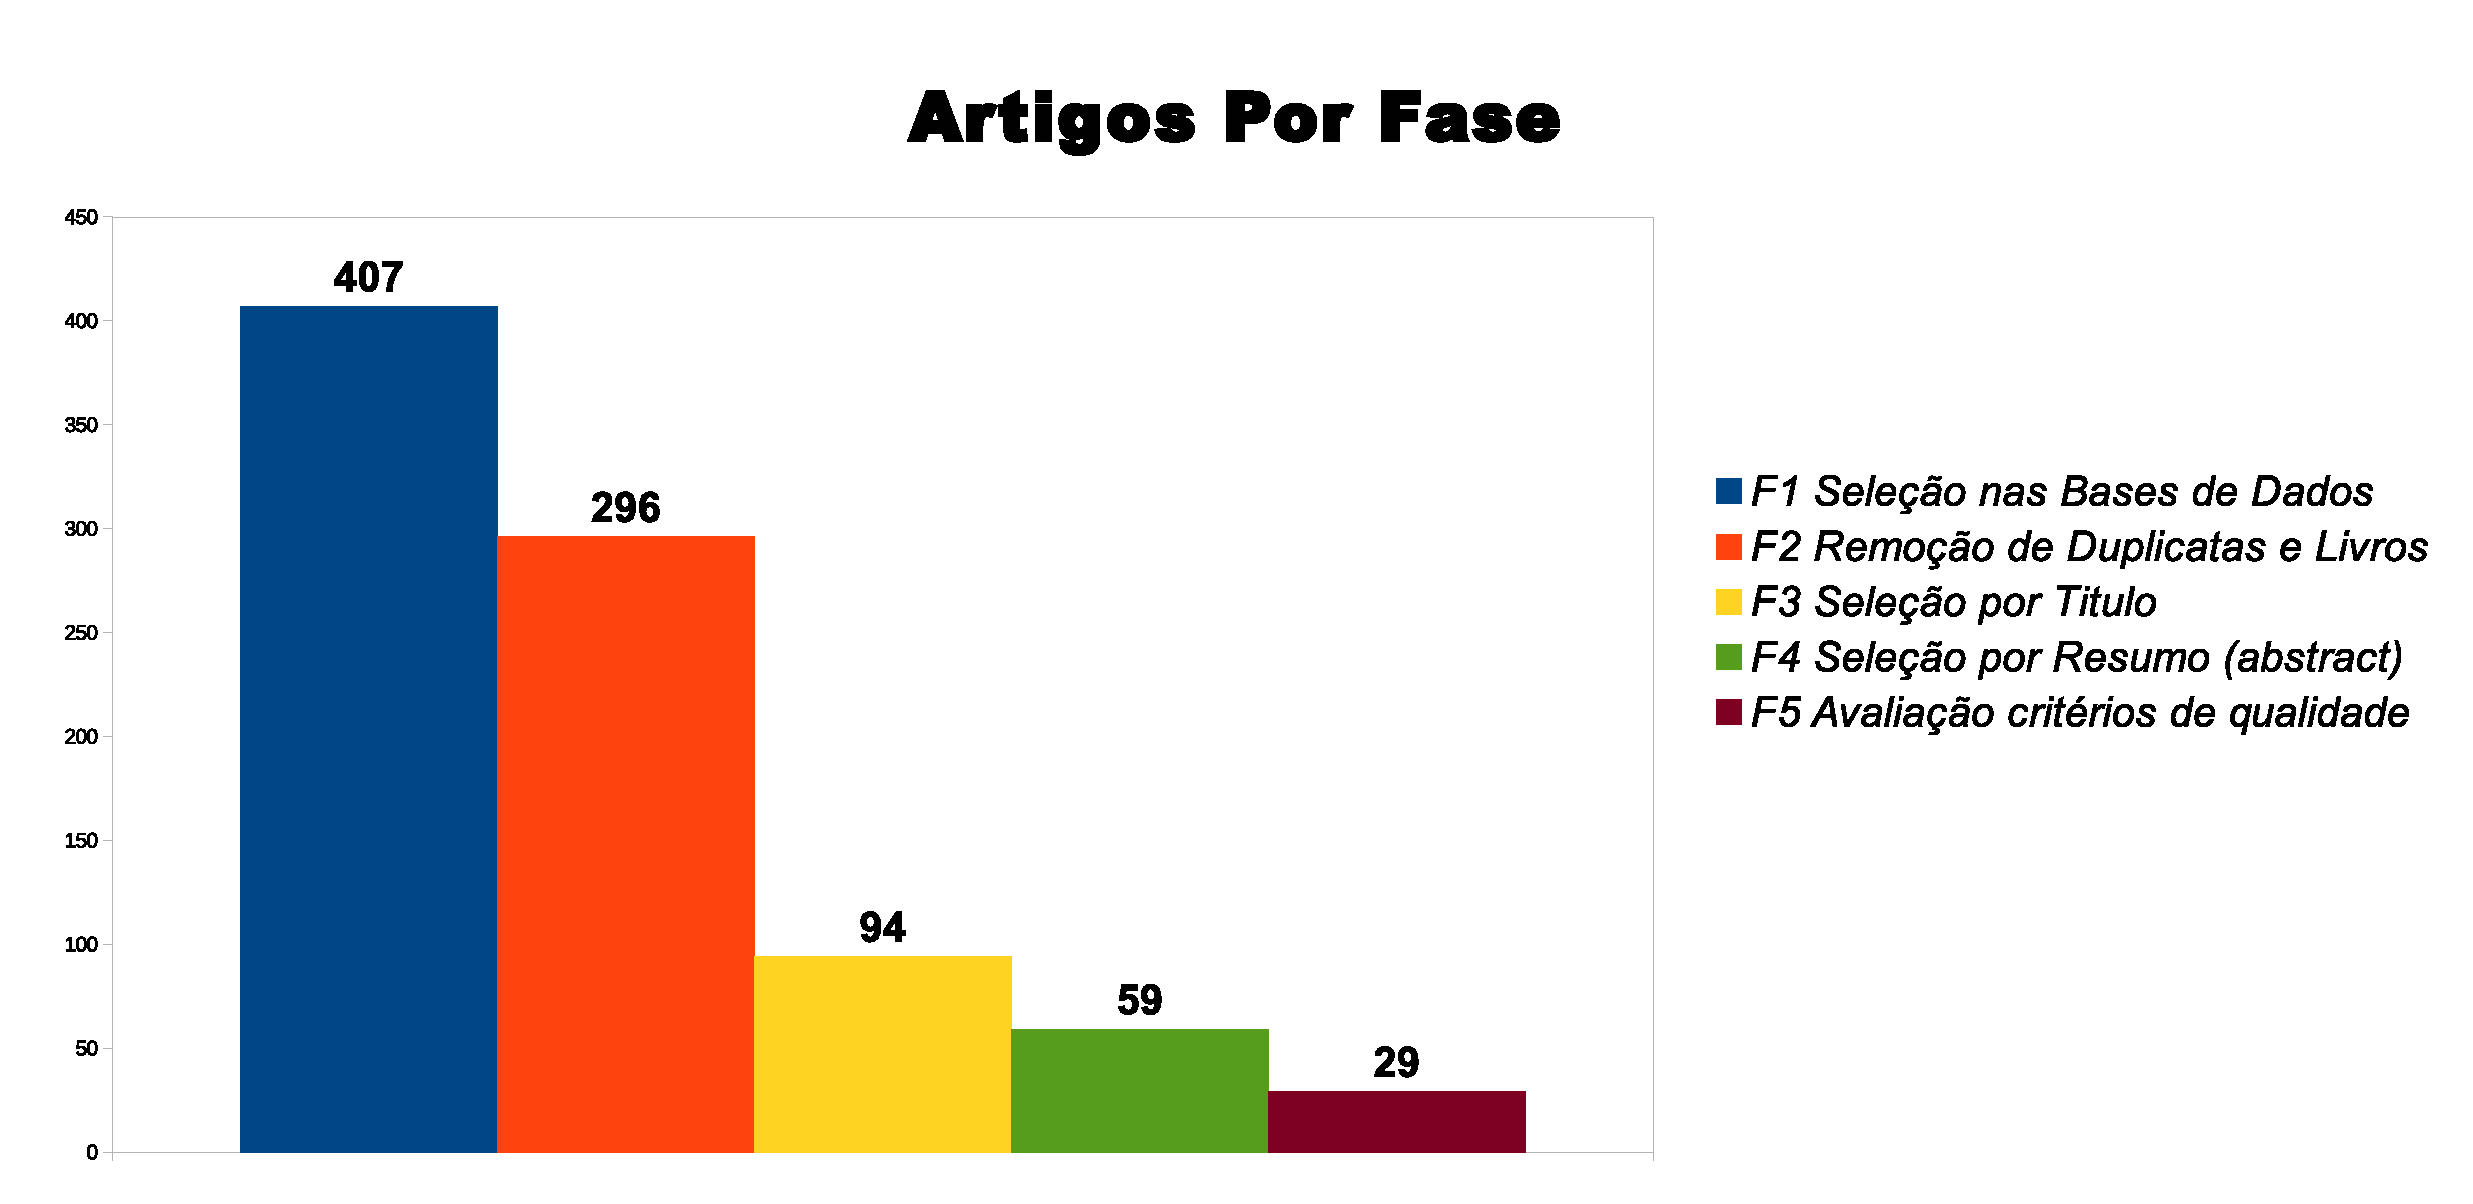
\includegraphics[width=\textwidth]{../img/graph_fases.eps}
\caption{Total de artigos em cada fase da SLR}%\label{fig:fases}
\end{figure}
\end{frame}
%%%%%%%%%%%%%%%%%%%%%%%%%%%%%%%%%%%%%%%%%%%%%%%%%%%%%%%%%

%%%%%%%%%%%%%%%%%%%%%%%%%%%%%%%%%%%%%%%%%%%%%%%%%%%%%%%%
\begin{frame}{Extração dos Dados}
    \begin{itemize}      \item Extração dos dados com base nos campos exibidos na Tabela
        \ref{tab:campos-form}.
      \item Validação única (sem pair-review)
    \end{itemize}

\begin{table}[ht]
\resizebox{9.5cm}{!}{%
\begin{tabular}{|c|l|l|}
\hline
\textbf{\#} & \multicolumn{1}{c|}{\textbf{Atributo}} & \multicolumn{1}{c|}{\textbf{Descrição}}                                                      \\ \hline
01          & Identificador do Estudo                & ID único para cada estudo, por exemplo IE01                                                  \\ \hline
02          & Data de Extração                       & Data no qual a extração foi conduzida (DD/MM/YYYY)                                           \\ \hline
03          & Nome do Extrator                       & Nome da pessoa responsável pela extração                                                     \\ \hline
04          & Autor                                  & Autor do estudo                                                                              \\ \hline
05          & Ano                                    & Ano de publicação do estudo                                                                  \\ \hline
06          & Título                                 & Título do Estudo                                                                             \\ \hline
07          & Tipo de Publicação                     & Artigo de journal ou conferência, dissertação, tese ou whitepaper                            \\ \hline
08          & Objetivo do Estudo                     & Quais foram os objetivos do estudo?                                                          \\ \hline
09          & Metodologia do Estudo                  & Quais foram as metodologias utilizadas no estudo?                                            \\ \hline
10          & Descobertas e Resultados               & Quais foram os resultados e descobertas do estudo                                            \\ \hline
11          & Nome da Ferramenta                     & Nome da ferramenta                                                                           \\ \hline
12          & Desenvolvedor                          & Pessoa ou empresa responsável pelo desenvolvimento                                           \\ \hline
13          & URL                                    & Site da internet da ferramenta                                                               \\ \hline
14          & Objetivo da Ferramenta                 & Qual funcionalidade principal da ferramenta                                                  \\ \hline
15          & Tipo de Arquitetura da Ferramenta      & Cliente/Servidor ou Web ou desktop                                                           \\ \hline
16          & Tipo de Licença da Ferramenta          & Software livre ou proprietário                                                               \\ \hline
17          & Avaliação da Ferramenta                & Como a ferramenta foi avaliada                                                               \\ \hline
18          & Estudo de Casos                        & Existe algum estudo de caso ou aplicação real da ferramenta                                  \\ \hline
19          & Ramo de Atuação                          & Qual setor da economia (governos, medicina, setor financeiro) a ferramenta já foi utilizada? \\ \hline
\end{tabular}
}
\caption{Campos do formulário de extração de dados}
\label{tab:campos-form}
\end{table}

\end{frame}
%%%%%%%%%%%%%%%%%%%%%%%%%%%%%%%%%%%%%%%%%%%%%%%%%%%%%%%%%

%%%%%%%%%%%%%%%%%%%%%%%%%%%%%%%%%%%%%%%%%%%%%%%%%%%%%%%%
\begin{frame}{Sintetização dos Dados}
    \begin{itemize}
       \item Neste trabalho o foco é na classificação e sumarização das
informações com o objetivo de responder as questões de pesquisa.
       \item Utilizado técnicas de \textit{Estatística Descritiva} conforme
         descrito por Wohlin et. al\cite{wohlin2012experimentation}
    \end{itemize}
\end{frame}
%%%%%%%%%%%%%%%%%%%%%%%%%%%%%%%%%%%%%%%%%%%%%%%%%%%%%%%%%

%%%%%%%%%%%%%%%%%%%%%%%%%%%%%%%%%%%%%%%%%%%%%%%%%%%%%%%%
\begin{frame}{Resultados}

    \begin{itemize}
      \item $Q1$: Quais são as ferramentas para
  Relatórios de Negócio que suportam a XBRL?
    \end{itemize}
\begin{table}[htb]
\resizebox{7.5cm}{!}{%
\begin{tabular}{|l|l|l|l|}
\hline
\multicolumn{1}{|c|}{\textbf{Nome da Ferramenta}} & \multicolumn{1}{c|}{\textbf{Desenvolvedor}} & \multicolumn{1}{c|}{\textbf{Arquitetura}} & \multicolumn{1}{c|}{\textbf{Licença}} \\ \hline
Abax XBRL                                         & 2H Software                                 & Framework                                 & Paga                                  \\ \hline
ADDACTIS Pillar3                                  & ADDACTIS                                    & Cliente/Servidor                          & Pago                                  \\ \hline
AGUILONIUS FactsConverter                         & Aguilonius                                  & Plugin Excel                              & Pago                                  \\ \hline
AGUILONIUS XBRL FACTORY SE                        & Aguilonius                                  & Cliente/Servidor                          & Paga                                  \\ \hline
AMANA SmartNotes                                  & AMANA SmartNotes                            & Desktop                                   & Paga                                  \\ \hline
Arele                                             & XBRL community                              & Framework                                 & Código Aberto                         \\ \hline
Batavia XBRL                                      & Batavia XBRL BV                             & Framework                                 & Paga.                                 \\ \hline
Calcbench                                         & Calcbench                                   & Web application                           & Paga                                  \\ \hline
DataTracks                                        & DataTracks                                  & Cliente/Servidor                          & Paga                                  \\ \hline
FinDynamics                                       & FinDynamics                                 & Excel Plugin                              & Paga                                  \\ \hline
FUJITSU Software Interstage XWand                 & Fujitsu                                     & Framework                                 & Paga                                  \\ \hline
Invoke e-Filing for Banks                         & Invoke                                      & Web Application                           & Paga                                  \\ \hline
IRIS Carbon                                       & IRIS Business Services Limited              & Cloud                                     & Paga                                  \\ \hline
Litix                                             & BR-AG                                       & Mobile                                    & Paga                                  \\ \hline
Oracle Hyperion Disclosure Management             & ORACLE                                      & Cliente/Servidor                          & Paga                                  \\ \hline
ParsePort XBRL Converter                          & ParsePort                                   & Web application                           & Paga                                  \\ \hline
ParsePort                                         & AltaNova                                    & Cliente/Servidor                          & Paga                                  \\ \hline
RegulatorWorks                                    & XBRLWorks                                   & Cliente/Servidor                          & Paga                                  \\ \hline
Reporting Standard XBRL                           & Reporting Standard                          & Desktop                                   & Paga                                  \\ \hline
Seahorse                                          & CoreFiling                                  & Cliente/Servidor                          & Paga                                  \\ \hline
Wdesk                                             & Workiva                                     & Web Application                           & Paga                                  \\ \hline
XBRL Processing Engine (XPE)                      & UBPartner                                   & Framework                                 & Paga                                  \\ \hline
xbrlOne Data Editor                               & Semansys Technologies                       & Desktop                                   & Paga                                  \\ \hline
XKUBED                                            & IPHIX                                       & Cliente/Servidor                          & Paga                                  \\ \hline
Yeti                                              & CoreFiling                                  & Web application                           & Paga                                  \\ \hline
XBRL Database Cluster                             & Argyris Argyrou , Andriy Andreev            & Cliente/Servidor                          & N/A                                   \\ \hline
XBRL Audit Assistant                              & Efrim Boritz \& Won Gyun No                 & Desktop                                   & N/A                                   \\ \hline
\end{tabular}
}
\caption{Ferramentas com Suporte à XBRL}
\label{tab:ferramentas}
\end{table}

\end{frame}
%%%%%%%%%%%%%%%%%%%%%%%%%%%%%%%%%%%%%%%%%%%%%%%%%%%%%%%%%
%%%%%%%%%%%%%%%%%%%%%%%%%%%%%%%%%%%%%%%%%%%%%%%%%%%%%%%%
\begin{frame}{$Q2$: Resultados}
    \begin{itemize}
      \item {$Q2$: Quais são as funcionalidades comuns as ferramentas
    que possibilitem a comparação entre elas?}
    \end{itemize}
\begin{figure}[htb]
\centering
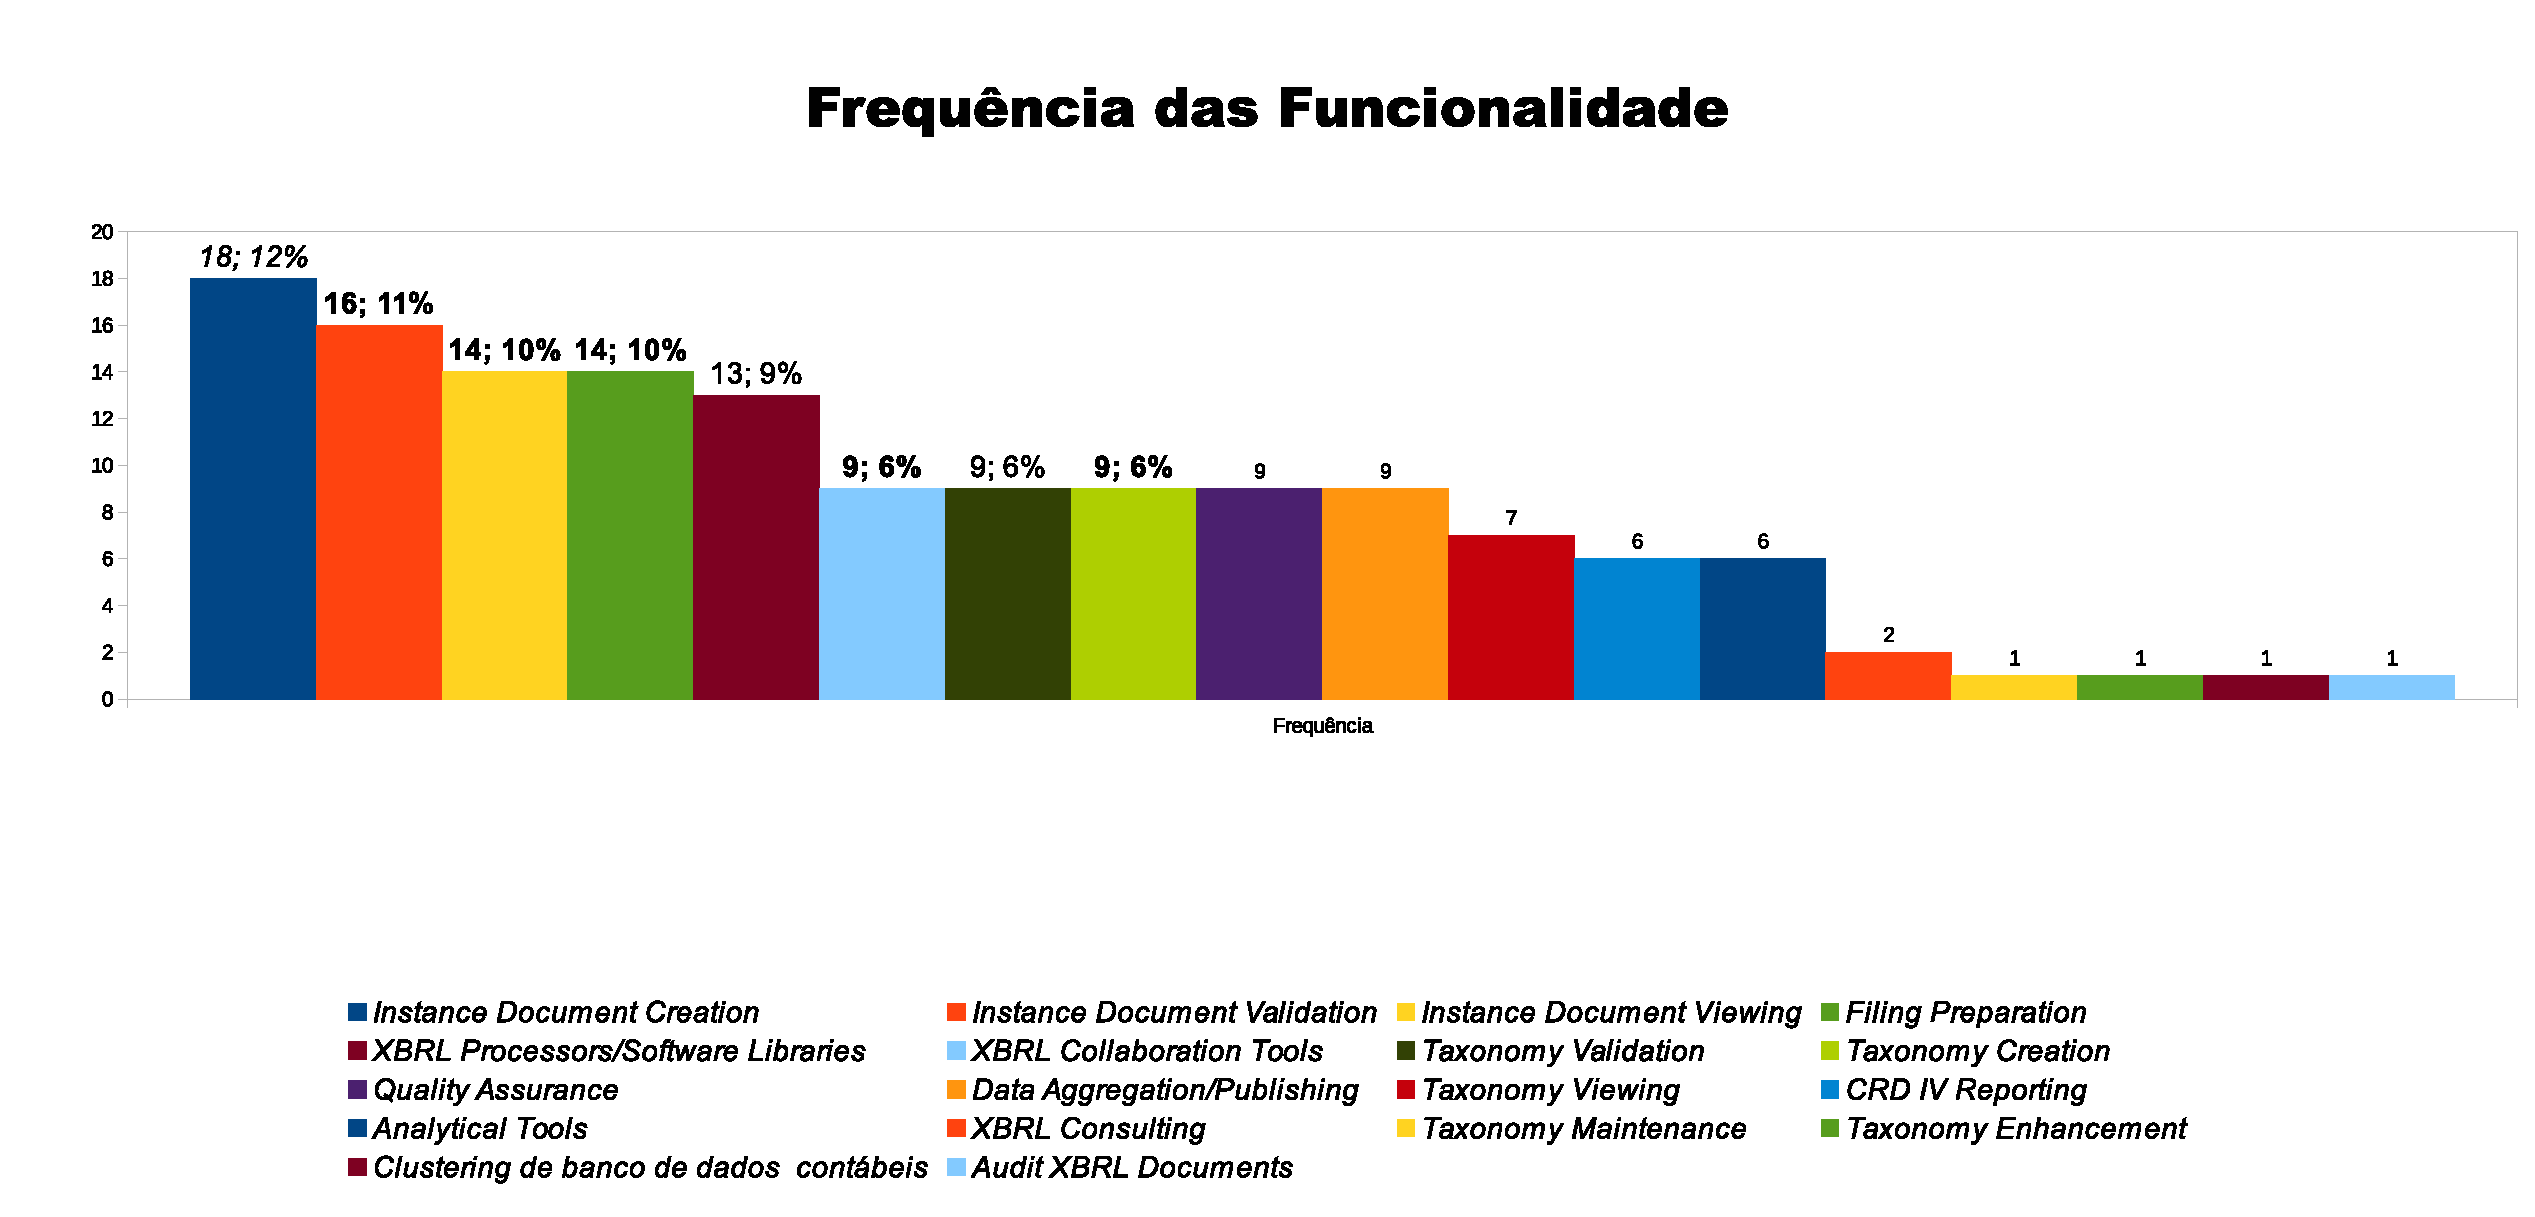
\includegraphics[width=.85\textwidth]{../img/graph_funcionalidades.eps}
\caption{Frequência das funcionalidades das ferramentas}
\label{fig:funcionalidades}
\end{figure}
\end{frame}
%%%%%%%%%%%%%%%%%%%%%%%%%%%%%%%%%%%%%%%%%%%%%%%%%%%%%%%%%
%%%%%%%%%%%%%%%%%%%%%%%%%%%%%%%%%%%%%%%%%%%%%%%%%%%%%%%%
\begin{frame}{Resultados}
    \begin{itemize}
         \item $Q3$: Existem casos reais de utilização da ferramenta
    (Estudos de Casos, Whitepapers e etc)?
         \begin{itemize}
               \item Não foi possível verificar nos estudos a avaliação prática das
        ferramentas.
              \item Há menções de clientes e de nichos de mercado no qual o sistema
        está inserido
              \item Não foi possível responder $Q3$
       \end{itemize}
    \end{itemize}
\end{frame}
%%%%%%%%%%%%%%%%%%%%%%%%%%%%%%%%%%%%%%%%%%%%%%%%%%%%%%%%%
%%%%%%%%%%%%%%%%%%%%%%%%%%%%%%%%%%%%%%%%%%%%%%%%%%%%%%%%
\begin{frame}{Resultados}
    \begin{itemize}
      \item $Q4$: Qual setor da economia
  (governos, medicina, setor financeiro) a ferramenta possui histórico de
  utilização?
    \end{itemize}

\begin{figure}[htb]
\centering
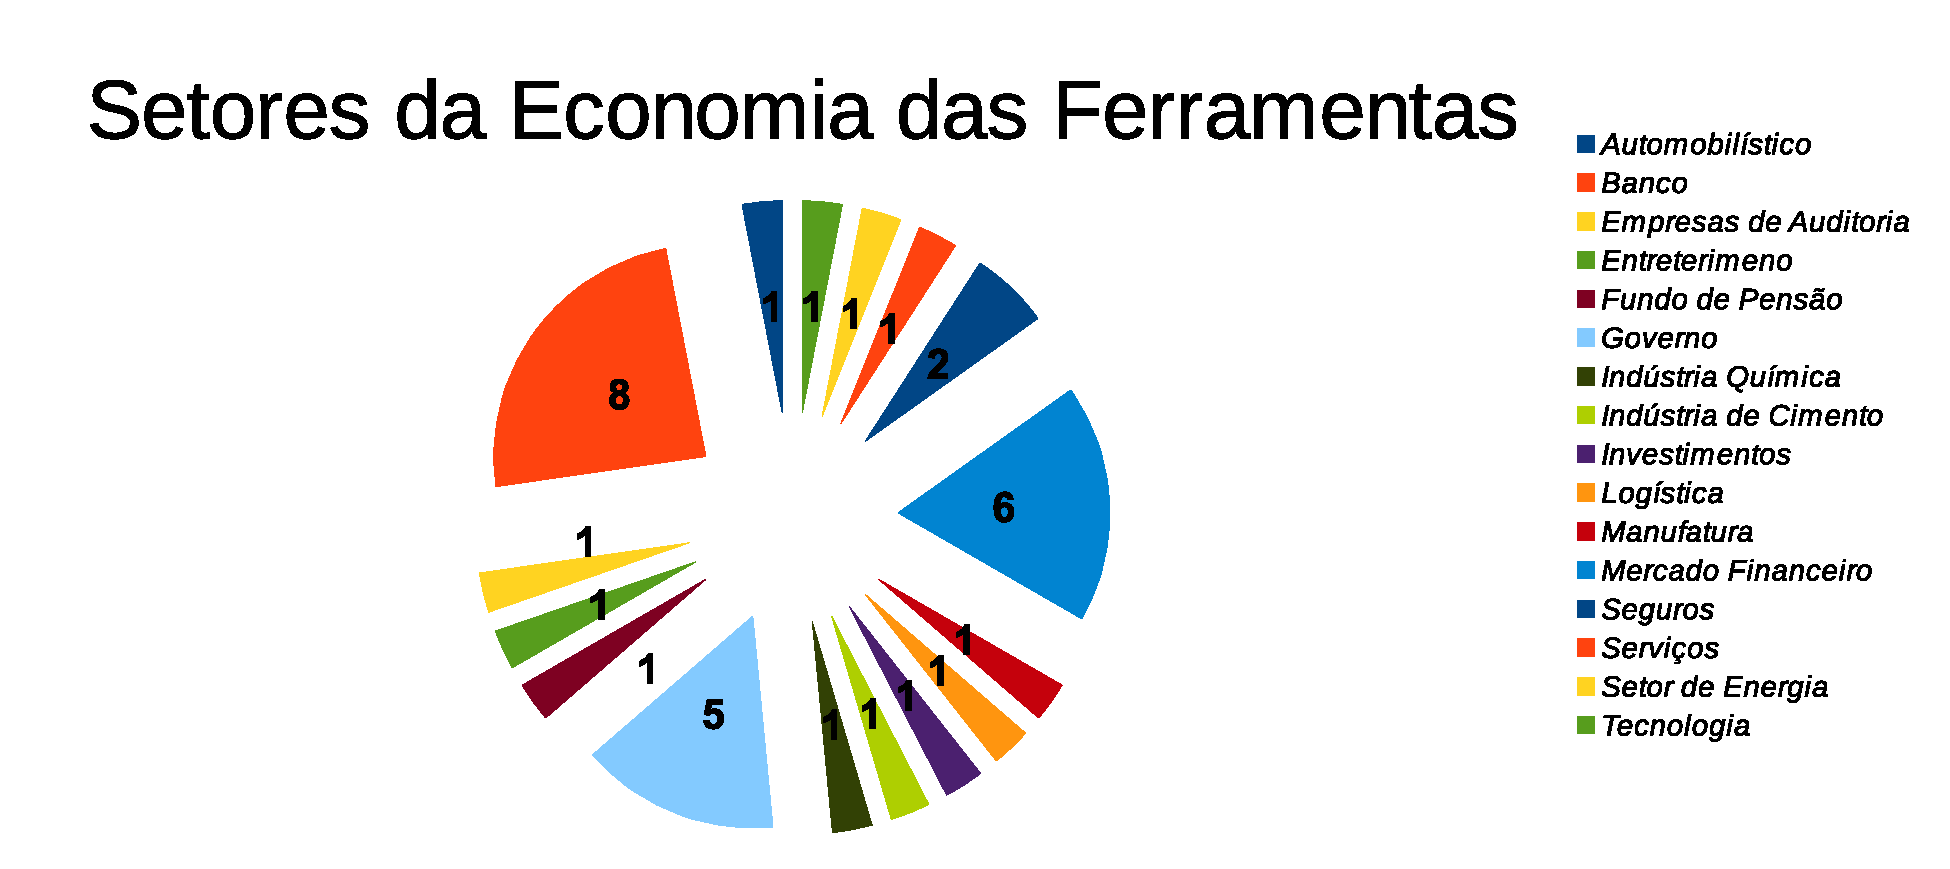
\includegraphics[width=.9\textwidth]{../img/graph_setores.eps}
\caption{Setores de Atuação das Ferramentas}
\label{fig:setores}
\end{figure}

\end{frame}
%%%%%%%%%%%%%%%%%%%%%%%%%%%%%%%%%%%%%%%%%%%%%%%%%%%%%%%%%
%%%%%%%%%%%%%%%%%%%%%%%%%%%%%%%%%%%%%%%%%%%%%%%%%%%%%%%%
\begin{frame}{Ameaças à Validade}
    \begin{itemize}
      \item Construção
        \begin{itemize}
        \item Definição das Questões de Pesquisa
        \end{itemize}
      \item Interna
        \begin{itemize}
        \item Inexistência de Pair Review
        \item Processo de Seleção
        \end{itemize}
      \item Externa
      \begin{itemize}
        \item Utilização de Gray Literature
        \end{itemize}
    \end{itemize}
\end{frame}
%%%%%%%%%%%%%%%%%%%%%%%%%%%%%%%%%%%%%%%%%%%%%%%%%%%%%%%%%
%%%%%%%%%%%%%%%%%%%%%%%%%%%%%%%%%%%%%%%%%%%%%%%%%%%%%%%%
\begin{frame}{Conclusão}
    \begin{itemize}
\item Revisão Sistemática da Literatura conforme proposto por Keele et al. \cite{keele2007guidelines}
\item SLR iniciou com 407 trabalhos que após seleção resultou em 29 estudos.
\item A partir destes estudos foi possível responder três das quatros questões de pesquisa propostas.

    \end{itemize}
\end{frame}
%%%%%%%%%%%%%%%%%%%%%%%%%%%%%%%%%%%%%%%%%%%%%%%%%%%%%%%%%
%%%%%%%%%%%%%%%%%%%%%%%%%%%%%%%%%%%%%%%%%%%%%%%%%%%%%%%%
\begin{frame}{Conclusão}
    \begin{itemize}
\item A maioria das ferramentas que dão suporte para funcionalidades mais
  básicas (criação, visualização e validação de objetos  de instância)
\item Predonimância nos setores financeiros e bancários
\item Possibilidade de Crescimento no setor público.
    \end{itemize}
\end{frame}
%%%%%%%%%%%%%%%%%%%%%%%%%%%%%%%%%%%%%%%%%%%%%%%%%%%%%%%%%
%%%%%%%%%%%%%%%%%%%%%%%%%%%%%%%%%%%%%%%%%%%%%%%%%%%%%%%%
\begin{frame}{Lições Aprendidas}
    \begin{itemize}
      \item Estudo piloto pode ajudar na definição das questões de pesquisa
      \item Processo de seleção de estudo primários pode ser melhorado
      \item Oportunidade para o desenvolvimento de ferramentas de suporte as SLR's
    \end{itemize}
\end{frame}
%%%%%%%%%%%%%%%%%%%%%%%%%%%%%%%%%%%%%%%%%%%%%%%%%%%%%%%%%
%%%%%%%%%%%%%%%%%%%%%%%%%%%%%%%%%%%%%%%%%%%%%%%%%%%%%%%%
\begin{frame}{Dúvidas}

\begin{figure}[htb]
\centering

\includegraphics[width=.5\textwidth]{../img/questions.jpg}
\end{figure}
\end{frame}
%%%%%%%%%%%%%%%%%%%%%%%%%%%%%%%%%%%%%%%%%%%%%%%%%%%%%%%%%
%%%%%%%%%%%%%%%%%%%%%%%%%%%%%%%%%%%%%%%%%%%%%%%%%%%%%%%%

\begin{frame}[allowframebreaks]
   \frametitle{Referências}
   \bibliographystyle{IEEEtranS}
   \bibliography{IEEEfull,bibliografia}
\end{frame}

\end{document}
